\documentclass[
	classe=$1^{ere}STI2D$,
]{évaluation}

\usepackage{tikz-repère}


\begin{document}

\title{Évaluation : dérivation (sujet A)}
\maketitle

\begin{exercice}
	Calculer les dérivées suivantes :
	\begin{enumerate}
		\item La dérivée de la fonction $f(x) = x - 1$ au point d'abscisse $3$.
		\item La dérivée de la fonction $f(x) = x² + 2$ au point d'abscisse $2$.
		\item La dérivée de la fonction $f(x) = -x² + 6x - 5$ au point d'abscisse $-1$.
	\end{enumerate}
\end{exercice}

\begin{exercice}
	Tracer les courbes de $x³$ et de sa dérivée entre $-3$ et $3$.

	(Remarque : il faudra prendre au moins $3$ unités par carreau en ordonnée)

	\correctionOr{
		\begin{center}
			\begin{tikzpicture}
				\tikzRepere{-3}{3}{-10}{10}[1][3]
				\draw[domain=-3:3,red] plot({\x},{1/3*\x*\x*\x});
				\draw[domain=-3:3,purple] plot({\x},{\x*\x});
				\node[red,right] at (-3,9) {$3x²$};
				\node[red,right] at (-3,-9) {$x³$};
			\end{tikzpicture}
		\end{center}
	}{}
\end{exercice}

\begin{exercice}

	Un motard accélère de manière continue sur une route, avant de se lancer dans les airs depuis une rampe.

	On modélise la situation par le schéma suivant :

	\begin{center}
		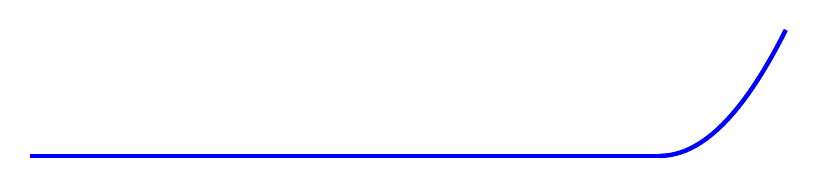
\begin{tikzpicture}[scale=0.8]
			\tikzRepere{-0.5}{18.5}{-0.5}{6.5}

			\draw[blue,ultra thick] (0,0) -- (10,0);
			\draw[blue,ultra thick,domain=10:12] plot({\x},{0.5*\x*\x - 10*\x + 50});

			\ifdefined\makeCorrection
				\draw[red,ultra thick,domain=12:17] plot({\x},{-0.5*\x*\x + 14*\x - 94});
			\fi
		\end{tikzpicture}
	\end{center}

	On admet que la position du motard est définie par la fonction $f$, telle que :
	\begin{itemize}
		\item Si $x∈[0 ; 10]$, le motard est sur la route, donc $f(x) = 0$.
		\item Si $x∈[10 ; 12]$, le motard est sur la rampe, dont la courbe est définie par $f(x) = \frac{1}{2}x² - 10x + 50$.
	\end{itemize}

	\begin{enumerate}
		\item Déterminer la pente de la rampe lorsque le motard la quitte.
		\item Si il n'y avait pas de gravité, quelle serait la hauteur du motard au point d'abscisse $20$ ?
		\item En prenant en compte la gravité, on admet que la position du motard après la rampe suit la courbe de la fonction $f(x) = -0,5x² + bx + c$, où $b$ et $c$ ne sont pas encore connus.
		      \begin{enumerate}
			      \item On admet que la fonction $f$ est dérivable sur l'intervalle $\intervalle{[}{0}{+∞}{[}$.

			            D'après la question $1$, quelle est la valeur de $f'(12)$ ?

			            On admet que sur l'intervalle $\intervalle{[}{12}{+∞}{[}$, la dérivée de $f$ peut s'écrire $f'(x) = -x + b$. Quelle est alors la valeur de $b$ ?

			            \correctionOr{{\color{red}$f'(12) = -12 + b = 2$, donc $b = 14$.}}{}
			      \item Lire sur le graphe la valeur de $f(12)$. En déduire la valeur de $c$.

			            \correctionOr{{\color{red}$f(12) = 2$, donc $f(12) = -72 + 14*12 + c = 2$, donc $c = -94$}}{}
		      \end{enumerate}
		\item Tracer alors la fonction $f(x) = -0,5x² + bx + c$ sur l'intervalle $[12;17]$.

		      À quelle abscisse le motard touche-il le sol ?
	\end{enumerate}
\end{exercice}

%=======================================================
%======================= SUJET B =======================
%=======================================================
\newpage
\setcounter{exercice}{1}

\title{Évaluation : dérivation (sujet B)}
\maketitle

\begin{exercice}
	Calculer les dérivées suivantes :
	\begin{enumerate}
		\item La dérivée de la fonction $f(x) = x + 2$ au point d'abscisse $3$.
		\item La dérivée de la fonction $f(x) = -x² + 1$ au point d'abscisse $2$.
		\item La dérivée de la fonction $f(x) = x² + 6x - 5$ au point d'abscisse $-1$.
	\end{enumerate}
\end{exercice}

\begin{exercice}
	Tracer les courbes de $x³$ et de sa dérivée entre $-3$ et $3$.

	(Remarque : il faudra prendre au moins $3$ unités par carreau en ordonnée)

	\correctionOr{
		\begin{center}
			\begin{tikzpicture}
				\tikzRepere{-3}{3}{-10}{10}[1][3]
				\draw[domain=-3:3,red] plot({\x},{1/3*\x*\x*\x});
				\draw[domain=-3:3,purple] plot({\x},{\x*\x});
				\node[red,right] at (-3,9) {$3x²$};
				\node[red,right] at (-3,-9) {$x³$};
			\end{tikzpicture}
		\end{center}
	}{}
\end{exercice}

\begin{exercice}

	Un motard accélère de manière continue sur une route, avant de se lancer dans les airs depuis une rampe.

	On modélise la situation par le schéma suivant :

	\begin{center}
		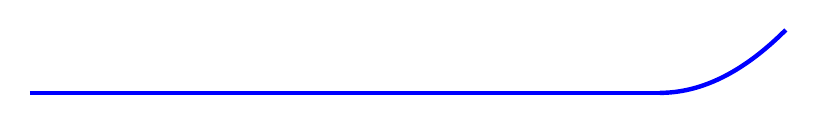
\begin{tikzpicture}[scale=0.8]
			\tikzRepere{-0.5}{18.5}{-0.5}{6.5}

			\draw[blue,ultra thick] (0,0) -- (10,0);
			\draw[blue,ultra thick,domain=10:12] plot({\x},{0.25*\x*\x - 5*\x + 25});

			\ifdefined\makeCorrection
				\draw[red,ultra thick,domain=12:17] plot({\x},{-0.25*\x*\x + 7*\x - 47});
			\fi
		\end{tikzpicture}
	\end{center}

	On admet que la position du motard est définie par la fonction $f$, telle que :
	\begin{itemize}
		\item Si $x∈[0 ; 10]$, le motard est sur la route, donc $f(x) = 0$.
		\item Si $x∈[10 ; 12]$, le motard est sur la rampe, dont la courbe est définie par $f(x) = \frac{1}{4}x² - 5x + 25$.
	\end{itemize}

	\begin{enumerate}
		\item Déterminer la pente de la rampe lorsque le motard la quitte.
		\item Si il n'y avait pas de gravité, quelle serait la hauteur du motard au point d'abscisse $20$ ?
		\item En prenant en compte la gravité, on admet que la position du motard après la rampe suit la courbe de la fonction $f(x) = -\dfrac{1}{4}x² + bx + c$, où $b$ et $c$ ne sont pas encore connus.
		      \begin{enumerate}
			      \item On admet que la fonction $f$ est dérivable sur l'intervalle $\intervalle{[}{0}{+∞}{[}$.

			            D'après la question $1$, quelle est la valeur de $f'(12)$ ?

			            On admet que sur l'intervalle $\intervalle{[}{12}{+∞}{[}$, la dérivée de $f$ peut s'écrire $f'(x) = -0,5x + b$. Quelle est alors la valeur de $b$ ?

			            \correctionOr{{\color{red}$f'(12) = -6 + b = 1$, donc $b = 7$.}}{}
			      \item Lire sur le graphe la valeur de $f(12)$. En déduire la valeur de $c$.

			            \correctionOr{{\color{red}$f(12) = 2$, donc $f(12) = -36 + 7*12 + c = 1$, donc $c = -47$}}{}
		      \end{enumerate}
		\item Tracer alors la fonction $f(x) = -0,5x² + bx + c$ sur l'intervalle $[12;17]$.

		      À quelle abscisse le motard touche-il le sol ?
	\end{enumerate}
\end{exercice}

\end{document}